\lab{Object Oriented Programming}{Object-Oriented Programming}
\label{lab:OOP}
\objective{Explain how to implement a GUI in python using PyQt.  Instruct how to create a basic GUI with standard features.}

\section*{Introduction}
\subsection*{Graphical User Interfaces and PyQt}
GUI stands for Graphical User Interface.  A GUI is an application that allows users to control a program through manipulation of graphical objects such as buttons, sliders, text boxes, and so forth.  In Python, we can use the PyQt toolkit to build GUIs.  From PyQt, we import the QtGui module which will allow us to implement the graphics as well as the interface itself. To demonstrate the main ideas behind building a GUI, we will create a simple program that displays inputted text. As you read, follow along by typing the code into a text editor and running it from your command line (use the command ''python filename.py''). Hands-on experience is the best way for GUI concepts to solidify. 

\subsection*{QMainWindow}
In this lab, a GUI will be made that we do some basic matrix operations such as calculating the determinant or inverse.  This GUI class will inherit from the QMainWindow class, which provides a main application window with support for useful things like a menu bar, toolbars, and animation.

\begin{lstlisting}
from PyQt4 import QtGui

class Printer(QtGui.QMainWindow):
	# This class inherits from the QWidget class found in the QtGui module.
	def __init__(self):
		# Call the __init__ method from QMainWindow, the class Printer is sub-classed from (its "super" class).
		super(Printer, self).__init__()
		self._initUI()
	
	def _initUI(self):
		# Our constructor
		self.show()

\end{lstlisting}

\subsection*{Creating Instance of GUI}
To launch the GUI, we need a main function which will run when the program is executed.  In the main function, we create an instance of the GUI in the following manner.  Note we must import sys in order to do this.
\begin{lstlisting}
import sys

if __name__== "__main__":
    app = QtGui.QApplication(sys.argv)
    p = Printer()
    sys.exit(app.exec_())
\end{lstlisting}

If we were to run the program at this point (using "python filename.py" in the terminal), a GUI instance would be created but there is no functionality of our GUI.  We first need to add widgets to our main window.

\section*{Widgets}
\emph{Widgets} are what make the magic happen in GUI's.
In Qt, widgets are objects that represent various elements of a GUI.
They keep track of drawing and refreshing the graphical display of the elements, abstracting the behavior of the elements, and defining ways to interact with other widgets.
When you push a button or enter text, widgets are what notice and respond accordingly.
In our \li{Printer} class, we will use \li{QLineEdit}, and \li{QLabel}, and \li{QPushButton}.

\subsection*{Organization}
We can organize our widgets on the screen using layouts.  A QHBoxLayout, for instance, allows you to align widgets horizontally, while a QVBoxLayout stacks them vertically.  You can also arrange them into grids of arbitrary dimensions using QGridLayout.  QMainWindow has a solitary central widget.  We will put our widgets into one layout, set that layout on a generic QWidget, and then assign that widget to the central widget.  In order to setup our GUI so that we can add widgets, we first add the following to our constructor: 
\begin{lstlisting}
def _initUI(self):
	# Creates the layout of the GUI.
	layout = QtGui.QVBoxLayout()

	# Creates a QWidget that we will use as our central widget.
	window = QtGui.QWidget()
	window.setLayout(layout)
	self.setCentralWidget(window)
\end{lstlisting}

\subsection*{Text Box}
In order to print out the results of the matrix calculation, we need a text box.  A text box can be added to the GUI by adding the following to the constructor:
\begin{lstlisting}
def _initUI(self):
	# Creates the output textbox and adds it to the layout.
	self.output = QtGui.QPlainTextEdit("Output here")
	layout.addWidget(self.output)
	
\end{lstlisting}


Note: Self is used to declare member variables.  You only need to declare an object with self if you intend to access that object from a member function of your class.  In this example, we do not declare the layouts with self because as soon as we assign the layout to the central widget we don't need to access them again.

\subsection*{Button}
Next we add a button to our GUI.  This will be done in a similar way as the text box.  We add the button to the constructor like the text box.
\begin{lstlisting}
# Creates a push button.
self.Button = QtGui.QPushButton("Enter")
layout.addWidget(self.Button)
\end{lstlisting}
At this point, the GUI has a text box and a button.  However, if the button is pressed, nothing happens.  We need to add functionality to our button and text box.
\subsection*{Add Functionality}
Now that we have our widgets, we need to tell them how to communicate.
Qt uses a system of \emph{signals} and \emph{slots}.
When a button is pushed or when text is entered, a widget throws a \emph{signal}.
We can specify which \emph{slot} catches the signal.
In this case, the signal being thrown is the text being entered in the text bar. We want a function that catches the signal, updates the displayed text, and clears the text bar.  In order to add functionality to the button, add the following to the constructor:
\begin{lstlisting}
self.Button.clicked.connect(self.clickButton)
\end{lstlisting}
\li{clickButton} is a method that will be declared inside the \li{Printer} class.  Once the button is pressed, the method clickButton will be called.  We will then set the text of the textbox to be ''Hello, World.''
\begin{lstlisting}
def clickButton(self):
	self.output.setPlainText("Hello, World")
\end{lstlisting}
\begin{problem}
Create a GUI with a button that will display your name in a text box once the button is pressed.
\label{prob:basicGUI}
\end{problem}

\section*{Important Widgets}

\subsection*{Menu Bar}
It is very common for GUIs to have a menu bar.  The QMainWindow class has a member function which generates one and puts it at the top of the window.  It will be empty to begin with.  We can add menu objects to it.  We can then add menus to the menus if we want, creating submenus to arbitrary levels.  At the bottom of the menu tree is an Action.  Action objects throw signals, and we connect the Actions to functions just like we did with the buttons.

\subsection*{Other Widgets}
Radio, table, spinbox, and QComboBox.

\begin{problem}
Complete the Matrix Calculator class that is provided in spec.py by
\begin{enumerate}
\item Adding a QComboBox to the GUI.
\item Add options to the QComboBox to calculate the determinant and inverse.
\item Implement the determinant and inverse function.  Hint: Use the standard NumPy commands.
\item Display the proper output in the textbox.
\end{enumerate}
\end{problem}

\section*{Documentation}
There are many different widgets that can be used in a variety of settings.  Here is a list of widgets and an explanation.  For a more comprehensive list of useful widgets see \href{http://doc.qt.io/qt-4.8/widgets-and-layouts.html}{link}.
For a really comprehensive list of widgets see \href{http://pyqt.sourceforge.net/Docs/PyQt4/qtgui.html}{link}.
\subsection*{Some More Useful Widgets}
Display picture, sliders, and spin box.
\begin{figure}
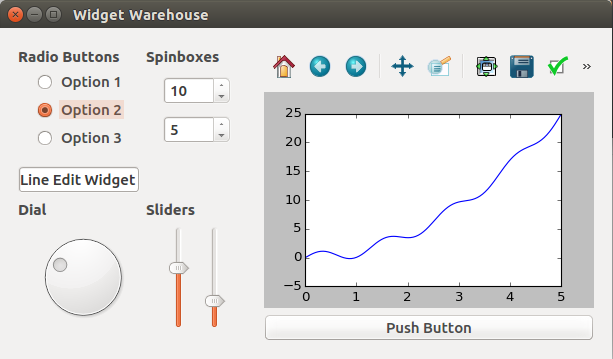
\includegraphics[width=\textwidth]{widgetwarehouse.png}
\caption{Here it is.}
\end{figure}

\begin{problem}
Create your own GUI.  You may make the GUI to display an old lab in an interesting way.  Some suggestions are Numerical Derivatives, Image Segmentation, SVD, or Convolution.  Or you may make your own GUI.  Include at least 5 widgets.
\end{problem}



\begin{lstlisting}
from PySide import QtGui, QtCore

class Printer(QtGui.QWidget):
	def __init__(self):
		super(Printer, self).__init__()
		# Call the _initUI function.
		self._initUI()
	
	def _initUI(self):
		'''Creates the widgets and tells them how to interact.'''
		
		# Create a class variable called textBar that is a QLineEdit widget.
		self.textBar = QtGui.QLineEdit()
		# Create a class variable called label that is a QLabel widget.
		self.label = QtGui.QLabel()

\end{lstlisting}



\begin{lstlisting}
from PySide import QtGui, QtCore

class Printer(QtGui.QWidget):
	def __init__(self):
		super(Printer, self).__init__()
		self._initUI()

	def _initUI(self):
		self.textBar = QtGui.QLineEdit()
		self.label = QtGui.QLabel()
		
		# When return is pressed in the textBar, it sends a signal and goes into the function updateText.
        # self.textBar accesses the textBar object.
        # returnPressed defines the inputted signal.
        # connect links the signal to the method later defined in this class: updateText.
		self.textBar.returnPressed.connect(self.updateText)
	
		
	def updateText(self):
	'''Updates what text is displayed and clears the textBar'''
		self.label.setText(self.textBar.displayText())
		self.textBar.clear()

\end{lstlisting}

Next, we need to set the layout and create a function that can be called from the command line.

\begin{lstlisting}
from PySide import QtGui, QtCore
import sys

class Printer(QtGui.QWidget):
	def __init__(self):
		super(Printer, self).__init__()
		self._initUI()

	def _initUI(self):
		self.textBar = QtGui.QLineEdit()
		self.label = QtGui.QLabel()
		
		self.textBar.returnPressed.connect(self.updateText)
	
		# Create a vertical box layout.
		# This will stack all widgets added to it vertically.
		vbox = QtGui.QVBoxLayout()
		# Add textBar as a widget and display it on the first row (0) in the first column (0).
        vbox.addWidget(self.textBar, 0, 0)
		vbox.addWidget(self.label, 1, 0)
		
		# Assemble the layout.
		self.setLayout(vbox)
		# Tell the dimensions of the vbox.
		# The first two numbers indicate placement on the screen while the second two represent the dimensions.
		self.setGeometry(50, 50, 200, 200)
		self.setWindowTitle("Simple Printer")
		self.show()
	
	def updateText(self):
		self.label.setText(self.textBar.displayText())
		self.textBar.clear()
		
def main():
	# Create a QApplication.
    # Note that if you are working in IPython Notebook, you need to restart your kernel before running the program, or a RuntimeError will occur.
	app = QtGui.QApplication(sys.argv)
	# Create a Printer object.
    # Since _initUI is called in the constructor, the GUI will appear and run.
	p = Printer()
	sys.exit(app.exec_())
if __name__ == "__main__":
	main()

\end{lstlisting}

\begin{problem}
Create a simple graphical user interface that will solve the quadratic formula given the necessary parameters.
Make the GUI look similar to the one below.
\begin{figure}[H]
\centering
\begin{comment}
\begin{subfigure}[b]{.49\textwidth}
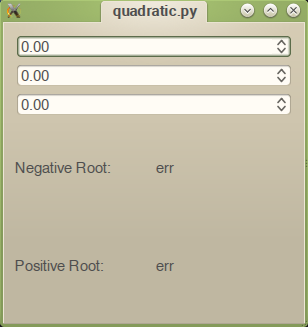
\includegraphics[width=\textwidth]{quadratic_view.png}
\end{subfigure}
\end{comment}
\begin{subfigure}[b]{.49\textwidth}
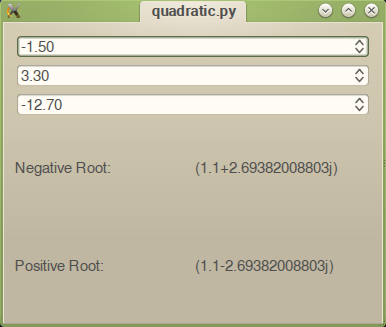
\includegraphics[width=\textwidth]{quadratic_view2.png}
\end{subfigure}
\end{figure}
The widgets that you will need are: \li{QDoubleSpinBox}, \li{QLabel}, \li{QGridLayout}, and \li{QVBoxLayout}. You may also want to import the cmath module in order to calculate complex solutions.
You can view the documentation for these classes, including all their methods and signals, at \url{http://qt-project.org/doc/qt-4.8/classes.html}
\label{prob:quadCalc}
\end{problem}


\section*{Specifications}

The following is a guideline for your solutions.

\begin{lstlisting}
import sys
from PySide import QtGui, QtCore

class People(object):
	pass
	
class ComplexNumber(object):
	pass
	
class QuadraticCalculator(QtGui.QWidget):
	pass
\end{lstlisting}